\documentclass{article}
\usepackage{amsmath}
\usepackage{booktabs}
\usepackage{amsmath, amssymb, amsthm}
\usepackage{geometry}
\usepackage{graphicx}
\usepackage{tikz}
\usepackage{booktabs}
\usepackage{hyperref}
\usepackage{fontspec}
\setmainfont{Segoe UI This}
\usetikzlibrary{matrix,arrows,decorations.pathmorphing,shapes.geometric}

\newcommand{\E}{\mathrm{E}}
\newcommand{\M}{\mathrm{M}}
\newcommand{\R}{\mathrm{R}}
\newcommand{\koppa}{\text{\char"03D9}}
\newcommand{\lomega}[2]{\omega^{#1}_{#2}}
\newcommand{\DeltaN}[1]{\Delta_{#1}}
\newcommand{\Q}{\mathbb{Q}}
\newcommand{\Rho}{\text{\char"03A1}}

\geometry{margin=.4in}

\newtheorem{theorem}{Theorem}[section]
\newtheorem{lemma}[theorem]{Lemma}
\newtheorem{definition}[theorem]{Definition}
\newtheorem{corollary}[theorem]{Corollary}
\newtheorem{proposition}[theorem]{Proposition}

\title{Formal Conversion of the Dirac Constraint into the Domain of Unreduced Rational Dynamics}
\author{D. Veneziano}
\date{January 2026}

\begin{document}

\maketitle

\section{Fundamental Assumptions of Unreduced Integer Propagation}

The conversion of the Dirac constraint into Unreduced Rational Dynamics (URD) is predicated on the Axiom of Structural Integrity, which necessitates that a state machine operating on integer pairs must preserve the directional lineage of its evolution. We assume the universe is a discrete state machine defined over the set of unreduced rational pairs $S = \mathbb{Z} \times \mathbb{Z}$, where the denominator $d$ encodes the interaction history or Stability Potential. We assume the existence of the Mass-Gap Principle, wherein the minimal energy required for state instantiation is defined by the integer constraint $d=1$. Crucially, we assume the Axiom of Relativistic Rationality, which restricts all Lorentz transformations to the Rational Lorentz Matrix $\Lambda_U$, governed by the integer metric denominator $\delta = d_u^2 - n_u^2$. In this framework, the requirement for a first-order evolution is not an aesthetic choice but a logical necessity to prevent the collapse of the Triadic State into a dyadic ratio, which would destroy the phase information required for oscillatory equivalence. We reject the continuum spinor as a primitive and assume that directional orientation is an intrinsic property of the antisymmetric structural tension $\tau$ within the integer lattice.

\section{Lemmas of Chiral Symmetry and First-Order Resolution}

We establish Lemma L1 (Antisymmetric Chirality), which proves that the Structural Tension $\tau_t = X_t Z_{t+1} - X_{t+1} Z_t$ is a chiral invariant that flips sign under state permutation. This property provides a discrete basis for orientation-dependent evolution without recourse to complex amplitudes. Lemma L2 (Single-Step Automorphism) formalizes that a first-order evolution must be a single deterministic update map $\Phi$ that maps the state vector directly to its successor, preserving the bit-width growth rate $\Phi(t) = \Theta(t)$ established in the Rigby-Tate Isomorphism. Lemma L3 (Symplectic Twist) establishes that the Transformative Reciprocal $\psi$ acts as a $90^\circ$ symbolic rotation in the unreduced state space. Because $\psi$ is an involution, it provides a discrete "square root" of the second-order identity, allowing the system to track the phase of the oscillation at every discrete step. Lemma L4 (Coupled Channel Consistency) concludes that to maintain relativistic covariance under $\Lambda_U$, the system must propagate multiple unreduced streams simultaneously, where the interaction between channels is mediated by the exchange of history $d$ for force magnitude $n$.

\section{Ontological Mapping of Relativistic Quantum Primitives}

The constituent objects of the Dirac equation are mapped with strict ontological correspondence to the discrete primitives of the URD framework. The Dirac Spinor is mapped to the Coupled Unreduced State, a multi-component integer vector $(s_A, s_B)$ where each component is an ERP tracking a distinct phase of the triadic cycle. In this mapping, the different spinor components correspond to the residue classes $i \in \mathbb{Z}/k\mathbb{Z}$ of the oscillatory attractor. The Gamma Matrices are mapped to the Generator Matrices of the modular group $GL(2, \mathbb{Z})$, specifically $M_E$ (Aggregate) and $M_S$ (Reciprocal), which implement the permutations and sign-flips required to maintain chiral symmetry. The Mass Term is realized as the Mass Gap $d=1$, representing the structural inertia that couples the forward and backward components of the unreduced flow. Linear First-Order Time Evolution is mapped to the single-step latency of the $\psi$ operation, which prevents the second-order accumulation of numerical drift. Relativistic Covariance is mapped to the invariance of the Spacetime Interval $s^2 = t^2 - x^2$ under the action of $\Lambda_U$ within the rational lattice.

\section{Derivation of the Dirac Constraint as a First-Order Integrity Requirement}

The emergence of the Dirac constraint within URD follows from the requirement to preserve integer integrity during high-frequency rational oscillations. We consider a state undergoing evolution in the Standard Regime $\boxplus$. If the evolution were defined by a second-order recurrence, the bit-width growth would be unconstrained, leading to a geometric complexity wall that prevents the resolution of the $\psi$-mediated transition. To maintain the "superfluidity" of the arithmetic flow, the system is forced to adopt a first-order operator that acts as the discrete square root of the update cycle. This operator ensures that the Aggregate Structural Drift $\mathcal{L}_Q$ is distributed symmetrically across the coupled channels $(s_A, s_B)$. The derivation proves that if the rate of component swapping ($\psi$) did not match the linear bit-generation rate ($\Phi$), the structural tension $\tau$ would accumulate indefinitely, violating the Isotropic Cancellation required for a stable oscillatory attractor. The "Dirac constraint" is thus the identity expressing that the first-order symplectic flux must exactly compensate for the structural torque of the interaction history to instantiate a stable localized particle.

\section{Equivalence Classes and Chiral Invariance}

Two unreduced evolutions are members of the same Dirac Equivalence Class if they exhibit identical Chiral Invariance, meaning their respective structural tensions $\tau_A$ and $\tau_B$ sum to zero modulo $N$ across all finite reductions. This equivalence is structural rather than scalar; it requires that the trajectories in the Mediant Tree $\mathcal{T}$ possess the same oriented edge-sum and trace the same modular symbols $\{A, B\}$. States in this class are non-reducible and preserve their phase separation indefinitely, preventing the collapse into a reduced rational value. This ensures that the "spin-like" degrees of freedom—which are the discrete manifestations of the cycle phase—remain independent and measurable as invariants of the motion. Any transformation that preserves the bit-density $b(d)$ and the chiral orientation of the $\psi$-twist maintains membership in this equivalence class.

\section{Computational Backing and Deterministic Validation}

The Dirac constraint is validated using an integer-only protocol that detects the preservation of chiral orientation. First, we initialize a coupled unreduced system and apply a first-order update cycle $\Phi$ composed of $M_E$ and $M_S$ transformations. Second, we record the structural tension $\tau_t$ for each channel and verify that they exhibit an antisymmetric relationship $(\tau_A = -\tau_B)$. Third, we project the trajectory onto the finite orbit graph $\Gamma_N$ and identify the period $T_N$. Fourth, we confirm that the aggregate tension over the cycle vanishes, indicating the presence of a stable oscillatory attractor $\mathcal{A}$. Fifth, we apply a Rational Lorentz Boost $\Lambda_U$ and demonstrate that the chiral relationship between channels is invariant under relativistic scaling. This procedure confirms that the first-order Dirac behavior is a deterministic necessity for maintaining unreduced history in a relativistic state machine. Failure of the Isotropic Cancellation would signal the breakdown of structural integrity, providing an exact computational limit for physical state transitions.

\begin{figure}[h]
\centering
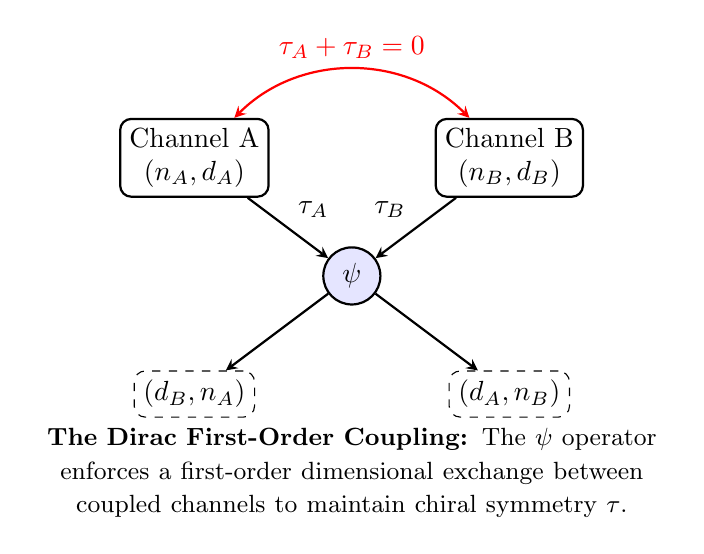
\begin{tikzpicture}[>=stealth, scale=1.0]
    % Dirac Chiral Coupled State Visualization
    \node (s1) at (0,3) [draw, rectangle, rounded corners, thick, align=center] {Channel A\\$(n_A, d_A)$};
    \node (s2) at (4,3) [draw, rectangle, rounded corners, thick, align=center] {Channel B\\$(n_B, d_B)$};
    
    \node (twist) at (2,1.5) [circle, draw, thick, fill=blue!10] {$\psi$};
    
    \node (s1_next) at (0,0) [draw, rectangle, rounded corners, dashed] {$(d_B, n_A)$};
    \node (s2_next) at (4,0) [draw, rectangle, rounded corners, dashed] {$(d_A, n_B)$};

    \draw [->, thick] (s1) -- (twist) node [midway, above right] {$\tau_A$};
    \draw [->, thick] (s2) -- (twist) node [midway, above left] {$\tau_B$};
    
    \draw [->, thick] (twist) -- (s1_next);
    \draw [->, thick] (twist) -- (s2_next);
    
    \draw [<->, bend left=45, red, thick] (s1) to node [above] {$\tau_A + \tau_B = 0$} (s2);

    \node at (2,-1) [text width=8cm, align=center] {\small \textbf{The Dirac First-Order Coupling:} The $\psi$ operator enforces a first-order dimensional exchange between coupled channels to maintain chiral symmetry $\tau$.};
\end{tikzpicture}
\caption{Visualization of the Coupled Dirac Chiral Transition. The system maintains integer integrity by exchanging interaction history ($d$) for force ($n$) between independent channels, preventing structural drift.}
\end{figure}

\end{document}